\section{Construcción del dataset y arquitectura del sistema}
\label{sec:dataset_arquitectura}

%
% Para citar: 
% 	(ver Sección~\ref{sec:dataset_arquitectura})
% 	como se describe en la Sección~\nameref{sec:dataset_arquitectura})
%

En este capítulo se describe el diseño, desarrollo e implementación del sistema responsable de generar el dataset empleado en el modelo de predicción de tráfico. Se parte de la identificación y análisis de las fuentes de datos disponibles, que incluyen mediciones de flujo vehicular, condiciones meteorológicas e incidencias viales. A continuación, se detallan las decisiones técnicas adoptadas en la arquitectura del sistema de integración, los patrones de diseño utilizados y el procedimiento empleado para consolidar todas las observaciones en una única estructura homogénea: la clase \texttt{MobilitySnapshot}. Finalmente, se justifican aspectos clave como la granularidad temporal del dataset, los criterios de selección de variables y las estrategias de persistencia.


\subsection{Fuentes de datos y análisis de disponibilidad}

Durante la primera fase del proyecto, se realizó un análisis exhaustivo de las fuentes de datos abiertas disponibles para la provincia de Bizkaia en el ámbito de los \acrshort{its}. La fuente de datos principal se corresponde con el API de Tráfico del portal de Open Data del Gobierno Vasco \cite{apiTraffic}. Se identificaron tres orígenes principales de datos:

\begin{itemize}
	\item \textbf{Gobierno Vasco}: mediante el API de Open Data Euskadi, se obtuvo información de aforos de tráfico e incidencias viales.
	\item \textbf{Ayuntamiento de Bilbao}: también a través de Open Data, se extrajeron series temporales de datos de tráfico en tiempo real.
	\item \textbf{Diputación Foral de Bizkaia}: al no disponer de un endpoint público, se logró contactar con los técnicos responsables y obtener acceso a sus datos mediante ficheros descargables proporcionados manualmente.
\end{itemize}

La cobertura de los datos obtenidos se representa en la tabla \ref{tab:cobertura_datos_opendata}, extraída y adaptada de la documentación técnica del repositorio del proyecto.

\begin{table}[H]
	\centering
	\caption{Cobertura de datos por fuente y tipo.}
	\label{tab:cobertura_datos_opendata}
	\renewcommand{\arraystretch}{1.2}
	\begin{tabularx}{\textwidth}{cXccc}
		\toprule
		\textbf{SourceId} & \textbf{Organización} & \textbf{Meters} & \textbf{Flows} & \textbf{Incidences} \\
		\midrule
		1 & Gobierno Vasco & \textcolor{mygreen}{\faCheck} & \textcolor{mygreen}{\faCheck} & \textcolor{mygreen}{\faCheck} \\
		2 & Diputación Foral de Bizkaia & \textcolor{gray}{\faHandPaper} & \textcolor{gray}{\faHandPaper} & \textcolor{mygreen}{\faCheck} \\
		3 & Diputación Foral de Álava & \textcolor{myred}{\faTimes} & \textcolor{myred}{\faTimes} & \textcolor{mygreen}{\faCheck} \\
		4 & Diputación Foral de Gipuzkoa & \textcolor{mygreen}{\faCheck} & \textcolor{myred}{\faTimes} & \textcolor{mygreen}{\faCheck} \\
		5 & Ayuntamiento Bilbao & \textcolor{mygreen}{\faCheck} & \textcolor{mygreen}{\faCheck} & \textcolor{mygreen}{\faCheck} \\
		6 & Ayuntamiento Vitoria-Gasteiz & \textcolor{mygreen}{\faCheck} & \textcolor{mygreen}{\faCheck} & \textcolor{mygreen}{\faCheck} \\
		7 & Ayuntamiento de Donostia-San Sebastián & \textcolor{mygreen}{\faCheck} & \textcolor{myred}{\faTimes} & \textcolor{mygreen}{\faCheck} \\
		\bottomrule
	\end{tabularx}
	
	\vspace{0.5em}
	\begin{itemize}
		\item \textcolor{mygreen}{\faCheck} Datos existentes y descargados correctamente.
		\item \textcolor{myred}{\faTimes} No existen datos para ese \texttt{sourceId} en OpenData.
		\item \textcolor{gray}{\faHandPaper} Datos obtenidos de forma externa e introducidos manualmente mediante programación.
	\end{itemize}
\end{table}

El caso de uso actual trata de cubrir la provincia de Bizkaia, por lo que únicamente van a ser necesarias las fuentes de datos con identificadores sourceId 1, 2 y 5.

Las incidencias se obtuvieron completamente para todos los sourceId.

En cuanto a la obtención de los datos meteorológicos, si bien es cierto que existe el API de meteorología del portal de Open Data del Gobierno Vasco \cite{apiMeteo}, éste presenta numerosos fallos a la hora de usarlo. Un claro ejemplo es la figura \ref{fig:euskalmet_api_error}. 

\begin{figure}[H]
	\centering
	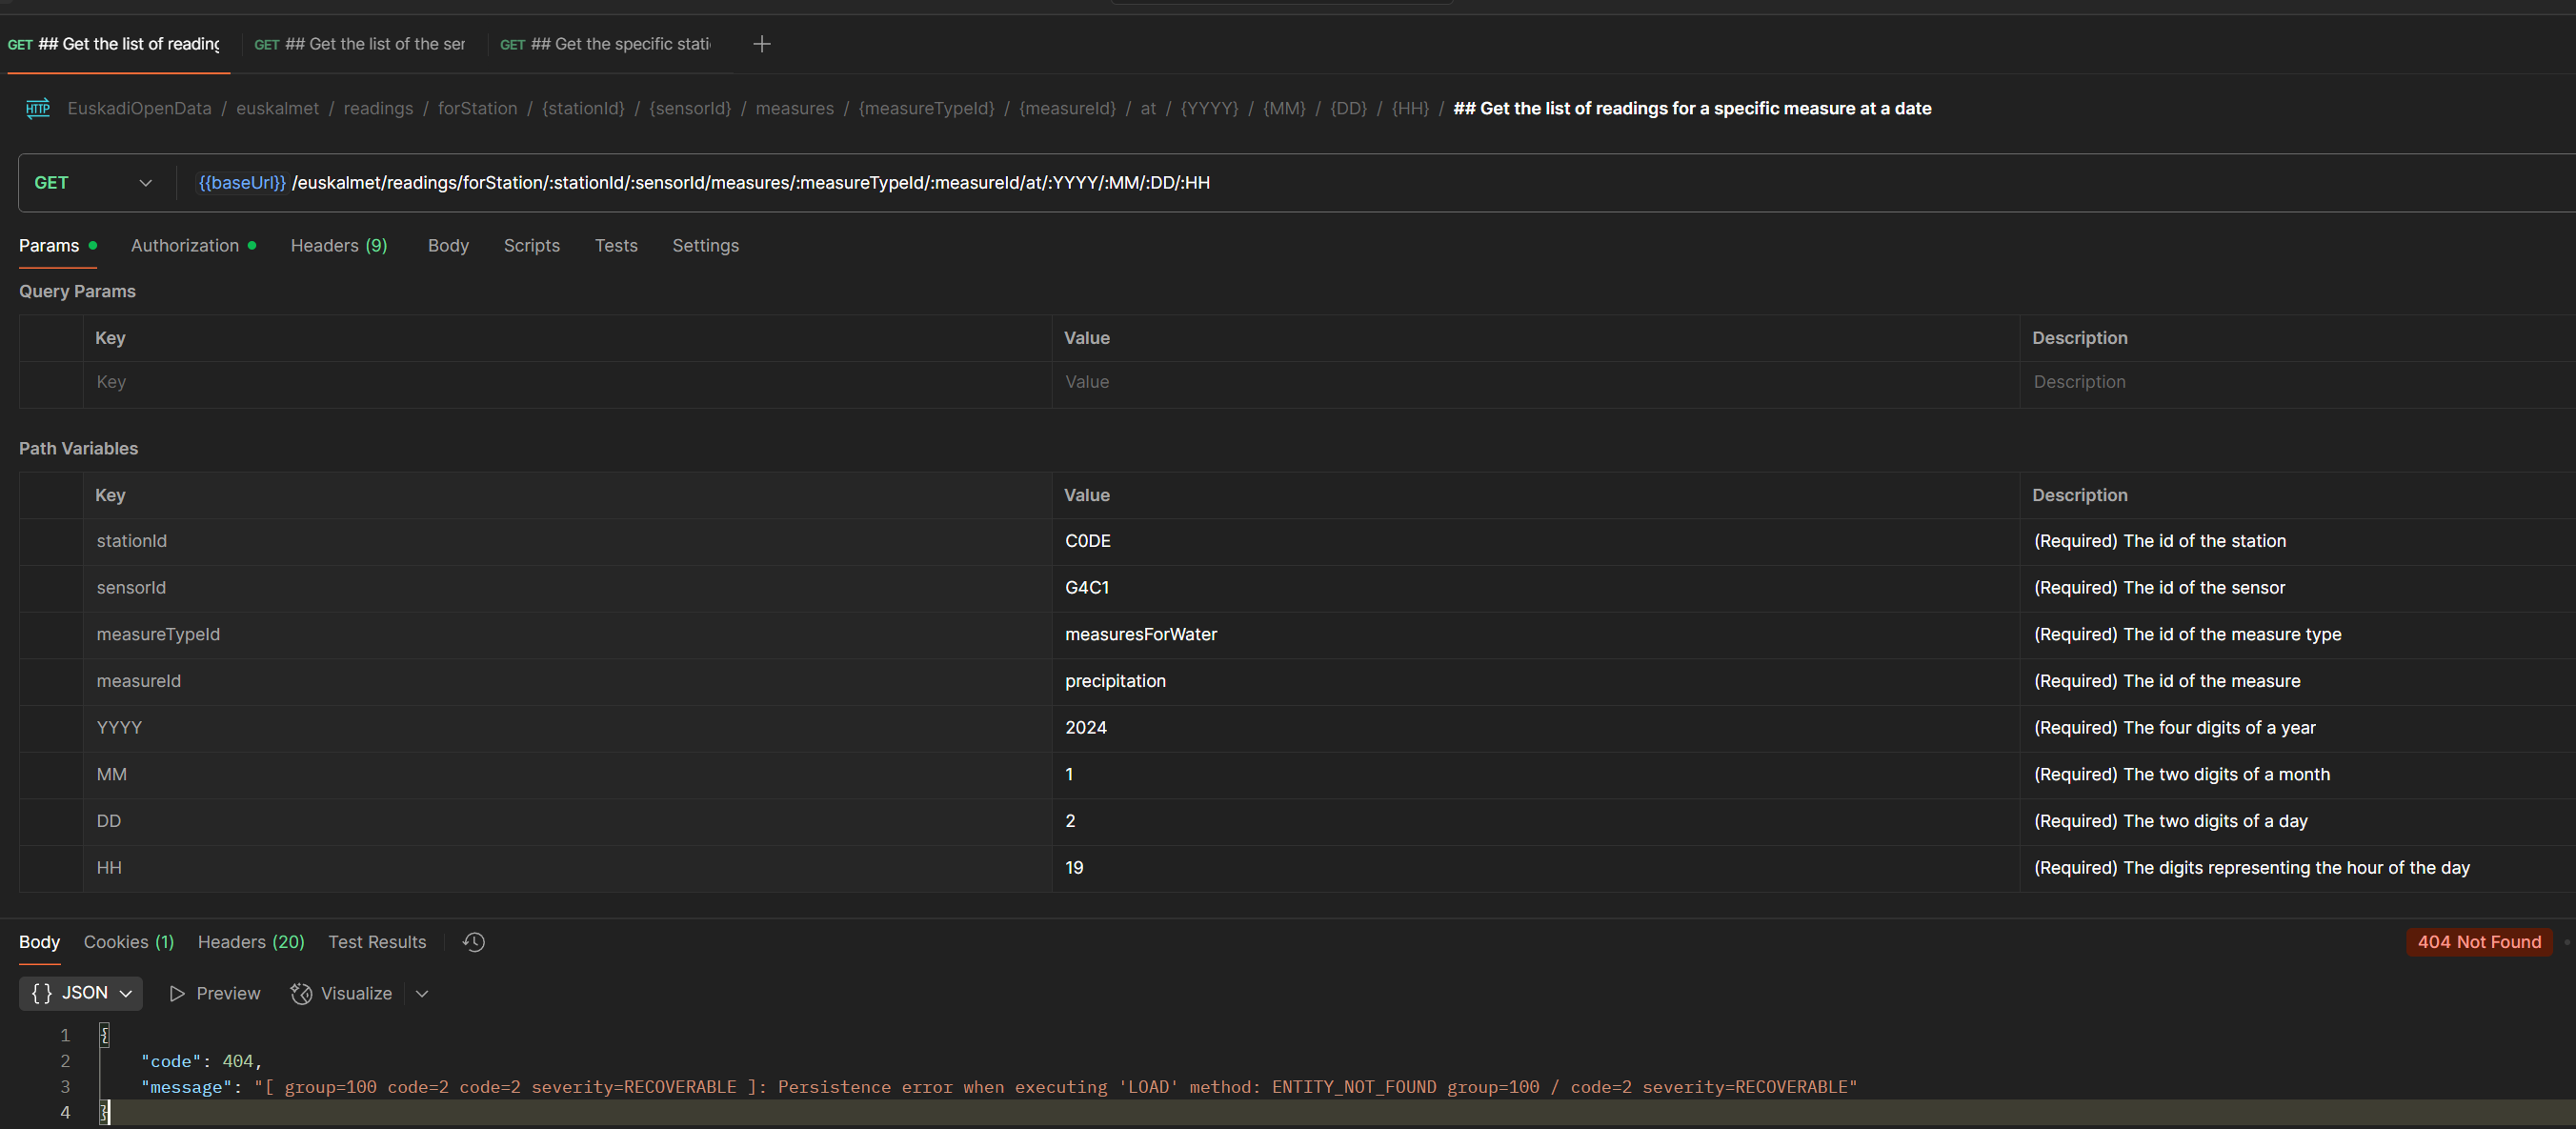
\includegraphics[width=0.95\textwidth]{includes/error_api_euskalmet.png}
	\caption{Ejemplo de error a la hora de consultar el API de Euskalmet.}
	\label{fig:euskalmet_api_error}
\end{figure}

Por ello, no se tenía la certeza de si se iban a obtener datos correctos, por lo que se pensó en maneras alternativas de obtener los propios datos. Así, en esa búsqueda de caminos se encontró, dentro del mismo portal de Open Data del Gobierno Vasco, las lecturas recogidas por las estaciones meteorológicas del año 2024 de forma bruta en formato XML, accesible a continuación \cite{xmlMeteo2024}. 

\subsubsection*{Modelo de datos almacenado}

Una vez explicadas las fuentes de datos, se podría comenzar a explicar cómo se van a almacenar dichos datos. En la figura \ref{fig:uml_classes} se puede ver las clases persistidas en la base de datos.

\begin{figure}[H]
	\centering
	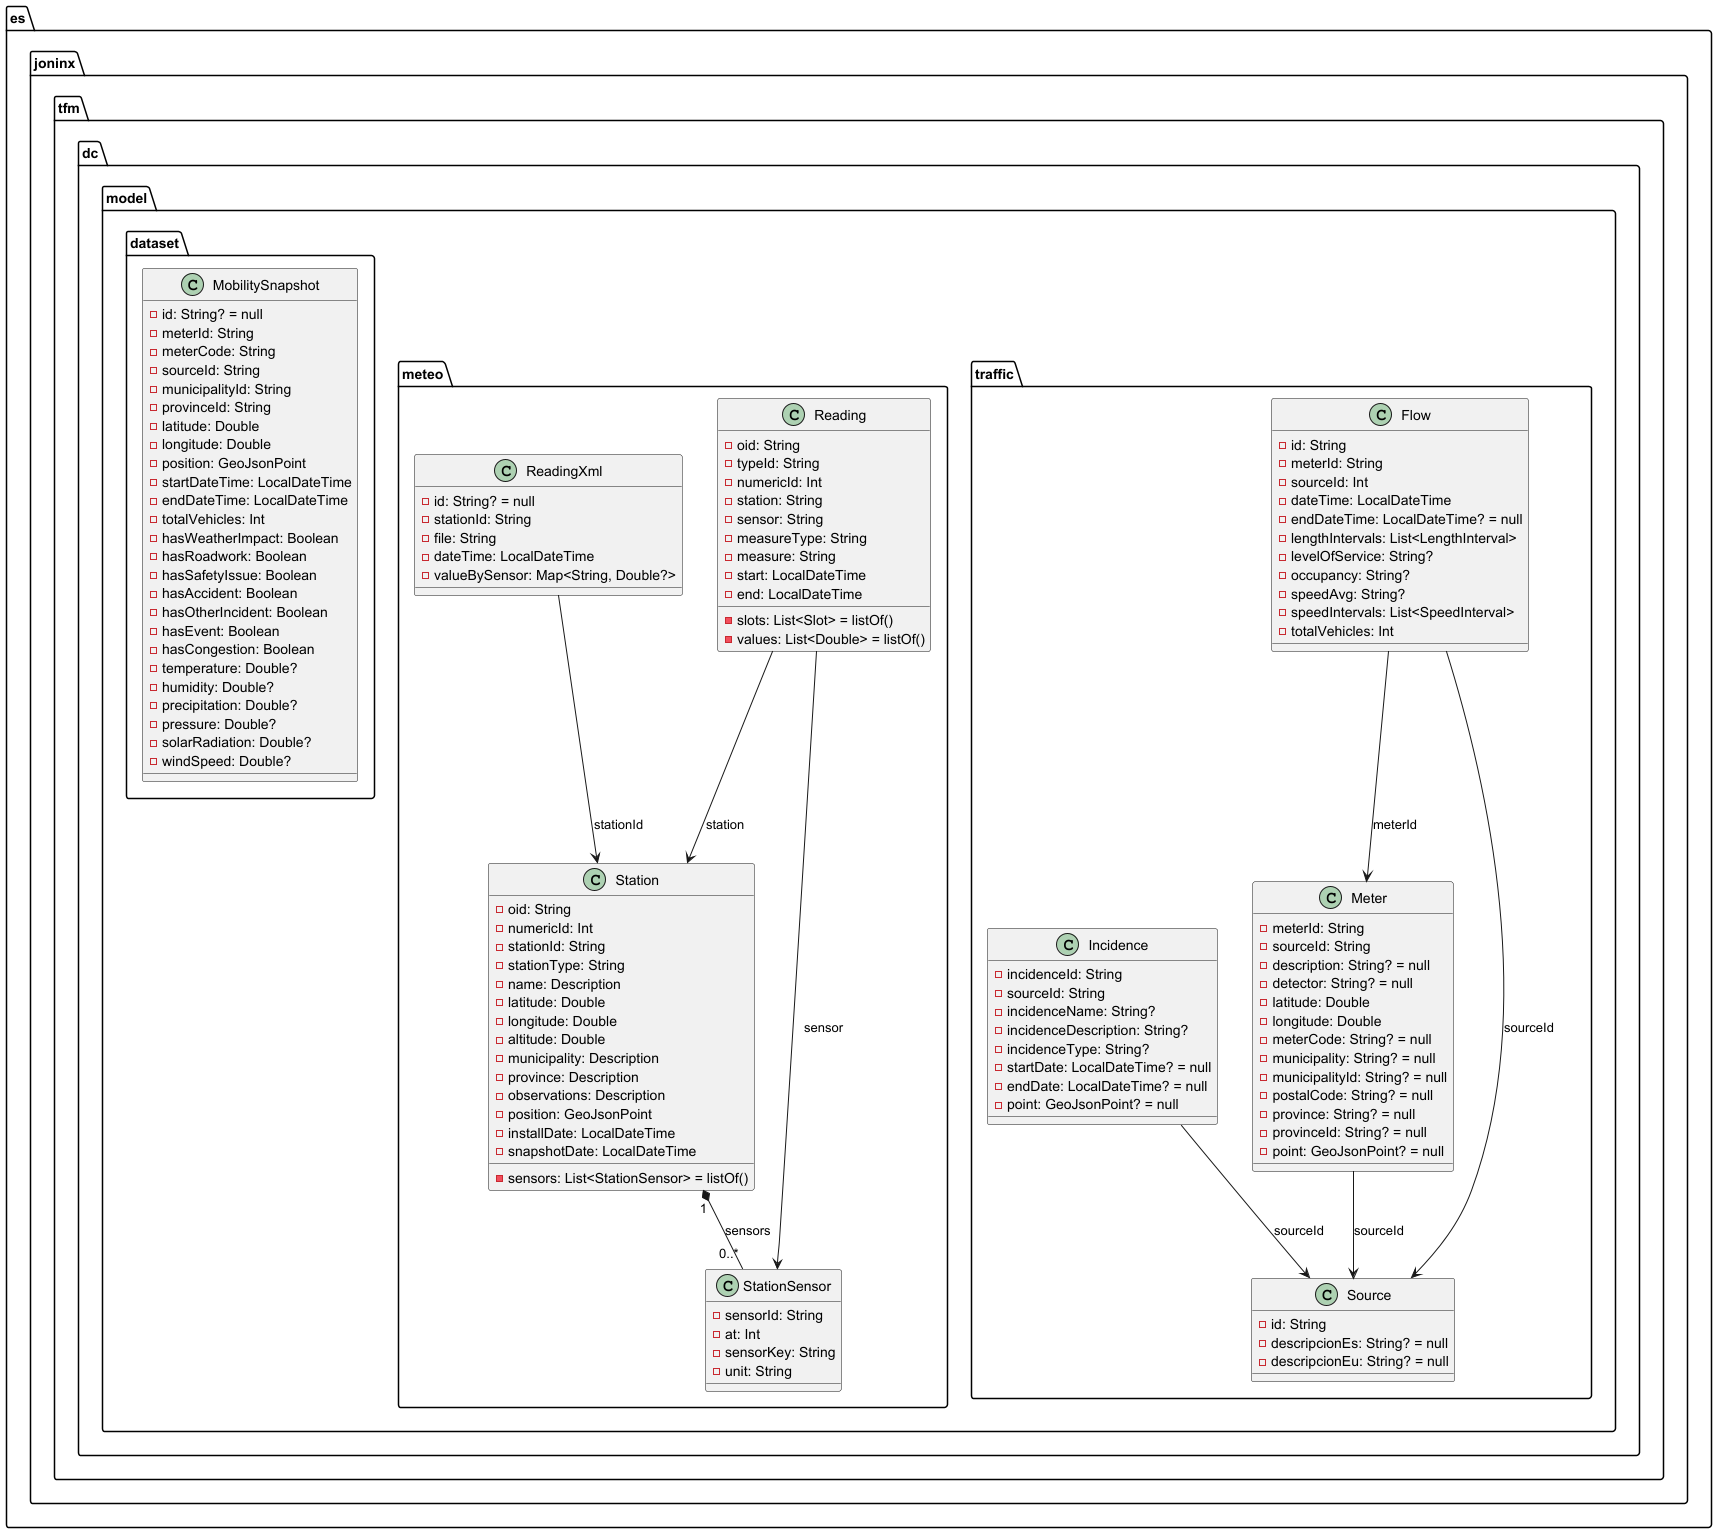
\includegraphics[width=0.95\textwidth]{includes/model_classes.png}
	\caption{Modelo de clases en UML de las entidades principales del sistema.}
	\label{fig:uml_classes}
\end{figure}

A continuación, se describen las entidades persistidas en base de datos, divididas por paquetes funcionales según su origen y propósito dentro del sistema: tráfico, meteorología y dataset resultante. Los datos de incidencias se incluyen dentro del paquete de tráfico, puesto que así viene encasillado en el API consultado. Cada clase representa un documento en la base de datos MongoDB, adaptado a una estructura flexible y orientada a documentos.

\paragraph{Flow}
Representa una medición de flujo de tráfico captada por un aforador en una fecha y hora determinadas. Entre sus atributos destacan:
\begin{itemize}
	\item \texttt{id}: identificador único del registro.
	\item \texttt{meterId}: identificador del aforador que ha generado la medición.
	\item \texttt{sourceId}: origen de los datos (Gobierno Vasco, Ayuntamiento, etc.).
	\item \texttt{dateTime} y \texttt{endDateTIme}: marca temporal de la medición. Puede que la marca de final no esté informada.
	\item \texttt{totalVehicles}: número total de vehículos detectados.
	\item \texttt{speedAvg}: velocidades medias de los vehículos detectados.
	\item \texttt{lengthIntervals} y \texttt{speedIntervals}: listas de intervalos por longitudes y velocidades, útiles para análisis más detallados. No se usa en este caso de uso.
\end{itemize}

\paragraph{Meter}
Contiene la información estática de los aforadores:
\begin{itemize}
	\item \texttt{meterId}, \texttt{sourceId}: identificadores del aforador y de la fuente de datos.
	\item \texttt{latitude}, \texttt{longitude} y \texttt{point}: ubicación geográfica. Útil el punto (tipo GeoJSON), puesto que es un índice geoespacial y se pueden realizar operaciones sobre el mismo (búsquedas por cercanía, distancias, etc).
	\item \texttt{postalCode}, \texttt{provinceId}, \texttt{municipalityId}: metadatos administrativos.
\end{itemize}

\paragraph{Incidence}
Recoge información sobre incidencias viales que pueden afectar al tráfico:
\begin{itemize}
	\item \texttt{incidenceId}, \texttt{sourceId}: identificadores del evento y de la fuente de datos.
	\item \texttt{incidenceName} e \texttt{incidenceDescription}: información descriptiva textual de la incidencia.
	\item \texttt{incidenceType}, \texttt{incidenceLevel}: tipificación normalizada para su posterior uso como variable categórica.
	\item \texttt{cause}, \texttt{road}, \texttt{pkStart}, \texttt{pkEnd}, \texttt{cityTown}, \texttt{province}, \texttt{autonomousRegion}, \texttt{carRegistration}: información adicional de la incidencia. Recoge datos como la carretera, los puntos kilométricos de inicio y de fin e información administrativa. No se tratará en este caso de uso.
	\item \texttt{startDate}, \texttt{endDate}: intervalo de vigencia de la incidencia. Esta información es relevante.
	\item \texttt{point}: ubicación geoespacial (tipo GeoJSON). Útil para realizar búsquedas por cercanía.
\end{itemize}

\paragraph{Source}
Representa los orígenes oficiales de datos, como el Gobierno Vasco o ayuntamientos. Sus campos identifican la organización y su descripción.

\vspace{1em}
\paragraph{Reading}
Es la clase principal para representar una lectura meteorológica horaria del API. Sin embargo, no se ha usado esta entidad para construir el dataset.
\begin{itemize}
	\item \texttt{oid}: identificador de la lectura.
	\item \texttt{typeId}: tipo de la lectura.
	\item \texttt{station}: estación meteorológica emisora.
	\item \texttt{sensor}: sensor responsable de la medición (\texttt{StationSensor}).
	\item \texttt{measureType} y \texttt{measure}: categorización de la medición.
	\item \texttt{start}, \texttt{end}: momento para el cual se ha realizado la medición.
	\item \texttt{slots}, \texttt{values}: forma en la que tiene el API de almacenar las mediciones. Cada elemento del slot se corresponde a un elemento de values, en la misma posición, indicando lo que se mide y su valor.
\end{itemize}

\paragraph{ReadingXml}
Clase específica para lecturas meteorológicas históricas extraídas desde ficheros XML. A diferencia de \texttt{Reading}, puede contener estructuras agrupadas por múltiples sensores. Es la clase definitiva empleada para construir el dataset.
\begin{itemize}
	\item \texttt{id}: identificador de la lectura.
	\item \texttt{stationId}: identificador de la estación meteorológica de la lectura.
	\item \texttt{file}: fichero de donde se ha extraído el dato de medición.
	\item \texttt{dateTime}: momento para el cual se ha realizado la medición.
	\item \texttt{valueBySensor}: forma en la que se almacenan las mediciones. El elemento clave identifica el tipo de medición y el valor indica el valor propio de la medición.
\end{itemize}

\paragraph{Station}
Define las estaciones meteorológicas que proporcionan las lecturas:
\begin{itemize}
	\item \texttt{stationId}: identificador único de la estación de medición.
	\item \texttt{name}, \texttt{municipality}, \texttt{province}: información administrativa.
	\item \texttt{latitude}, \texttt{longitude}, \texttt{altitude} y \texttt{position}: coordenadas geográficas.
	\item \texttt{sensors}: lista de sensores instalados.
\end{itemize}

\paragraph{StationSensor}
Define la configuración física de un sensor en una estación:
\begin{itemize}
	\item \texttt{sensorId}, \texttt{sensorKey}: clave de sensor y código técnico.
	\item \texttt{unit}, \texttt{at}: unidad de medida y altura del sensor (en centímetros).
\end{itemize}

\vspace{1em}
\paragraph{MobilitySnapshot}
Es la entidad clave que representa un punto de datos enriquecido para el modelo predictivo. Cada snapshot incluye:
\begin{itemize}
	\item \texttt{id}: identificador único del dato.
	\item \texttt{meterId}, \texttt{meterCode}: información identificativa del aforador del cual se ha extraído la información de Flow.
	\item \texttt{totalVehicles}: indica la cantidad de vehículos que han pasado por este punto entre en el espacio temporal definido.
	\item \texttt{latitude}, \texttt{longitude}, \texttt{position}: información geoespacial del snapshot. Nótese que el campo positión es de tipo GeoJson.
	\item \texttt{startDateTime}, \texttt{endDateTime}: indica entre qué momentos es válido este snapshot.
	\item \texttt{hasAccident}, \texttt{hasWeatherImpact}, \texttt{hasConstruction}, etc: indica si durante este espacio temporal cerca de este punto ha ocurrido alguna incidencia del tipo.
	\item \texttt{temperature}, \texttt{humidity}, \texttt{windSpeed}, \texttt{solarRadiation}, \texttt{pressure}, etc: indica los valores meteorológicos del propio snapshot.
\end{itemize}

Esta clase es el resultado final del proceso de integración de datos y constituye la base sobre la que se entrena el modelo de predicción de tráfico.

\subsection{Recolección, arquitectura y patrones de diseño empleados}

El software encargado de la recolección de datos se ha desarrollado en \textbf{Kotlin con Spring Boot}, aplicando principios de arquitectura hexagonal y múltiples patrones de diseño para garantizar su mantenibilidad y robustez. Entre los patrones de diseño empleados destacan:

\begin{itemize}
	\item \textbf{Builder}: utilizado en la generación del dataset a través de la clase \texttt{MobilitySnapshotBuilder}.
	\item \textbf{Repository}: todas las operaciones de acceso a datos (\texttt{FlowRepository}, \texttt{MeterRepository}, etc.) se abstraen en repositorios desacoplados.
	\item \textbf{Service Layer}: la lógica de negocio reside en servicios como \texttt{FlowService}, \texttt{MeterService}, \texttt{IncidenceService}.
	\item \textbf{DTO (Data Transfer Object)}: se emplean DTOs para el intercambio de datos entre capas, evitando el acoplamiento con los modelos de persistencia.
	\item \textbf{Helper/Utility Classes}: utilidades para parseo, validación y transformación de datos (por ejemplo, para el tratamiento de ficheros XML meteorológicos).
	\item \textbf{Facade}: fachadas que agrupan operaciones complejas en interfaces sencillas, facilitando la integración con servicios externos.
	\item \textbf{Factory} y \textbf{Singleton}: empleados para instanciar objetos según el origen de datos y para servicios centrales, respectivamente.
\end{itemize}

El sistema de integración y procesamiento de datos ha sido desarrollado en Kotlin, un lenguaje moderno que combina características orientadas a objetos y funcionales. La clase \texttt{MobilitySnapshotGeneratorService}, pieza central del sistema, hace uso de varias construcciones idiomáticas que representan buenas prácticas del lenguaje y potencian la expresividad, la seguridad y la eficiencia en tiempo de desarrollo.

A continuación se destacan las características más reseñables del uso de Kotlin en dicha implementación:

\begin{itemize}
	\item \textbf{Inferencia de tipos}: permite declarar variables sin especificar explícitamente su tipo cuando este es deducible por el compilador, lo que mejora la legibilidad. Por ejemplo:
	\begin{lstlisting}[language=Kotlin]
		val intervals = mutableListOf<Pair<LocalDateTime, LocalDateTime>>()
	\end{lstlisting}
	
	\item \textbf{Funciones de orden superior y operadores de colección}: se hace uso extensivo de funciones como \texttt{mapNotNull}, \texttt{groupBy}, \texttt{sumOf}, y \texttt{forEachIndexed}, lo que refleja el paradigma funcional del lenguaje.
	\begin{lstlisting}[language=Kotlin]
		val groupedByMeter = flows.groupBy { it.meterId }
		val snapshots = groupedByMeter.mapNotNull { (meterId, flowList) -> ... }
	\end{lstlisting}
	
	\item \textbf{Acceso seguro a valores opcionales con \texttt{let}}: se utiliza para gestionar accesos a valores almacenados en cachés evitando estructuras condicionales explícitas.
	\begin{lstlisting}[language=Kotlin]
		meterToStationCache[meterId]?.let {
			log.debug("Cache HIT: meterId=$meterId → stationId=$it")
			return it
		}
	\end{lstlisting}
	
	\item \textbf{Operador Elvis (\texttt{?:})}: permite proporcionar valores por defecto ante posibles nulos, mejorando la seguridad frente a \texttt{NullPointerException}.
	\begin{lstlisting}[language=Kotlin]
		val meters = meterRepository.findAllBySourceIdIn(sourceIds)
		.collectMap { it.meterId }
		.block() ?: emptyMap()
	\end{lstlisting}
	
	\item \textbf{Lambdas expresivas y destructuración de pares}: se utilizan para recorrer colecciones de forma clara, aprovechando las capacidades de Kotlin para trabajar con estructuras complejas.
	\begin{lstlisting}[language=Kotlin]
		intervals.forEachIndexed { idx, (intervalStart, intervalEnd) -> ... }
	\end{lstlisting}
	
	\item \textbf{Inyección de dependencias vía constructor}: siguiendo los principios de inversión de dependencias (en otras palabras, un término que mezcla los conceptos de Inyección de Dependencias e Inversión de Control), se definen todos los componentes del servicio a través del constructor primario.
	\begin{lstlisting}[language=Kotlin]
		class MobilitySnapshotGeneratorService(
		private val cfg: Cfg,
		private val snapshotBuilder: MobilitySnapshotBuilder,
		...
		)
	\end{lstlisting}
	
	\item \textbf{Uso de \texttt{companion object} para logging}: se emplea una instancia estática del logger utilizando el enfoque idiomático del lenguaje.
	\begin{lstlisting}[language=Kotlin]
		companion object {
			val log: Logger = LogManager.getLogger(this::class.java)
		}
	\end{lstlisting}
	
	\item \textbf{Uso responsable de colecciones mutables}: aunque se utilizan listas mutables para la generación de intervalos y resultados temporales, estas estructuras se manejan de forma controlada y local, siguiendo las recomendaciones del lenguaje.
\end{itemize}

El uso de estas características idiomáticas refleja una implementación robusta, alineada con las buenas prácticas modernas del ecosistema Kotlin, y facilita tanto el mantenimiento del código como su extensibilidad futura.

La decisión de utilizar una base de datos \textbf{NoSQL, MongoDB}, responde a la necesidad de trabajar con estructuras flexibles, heterogéneas y de gran volumen, propias del contexto del proyecto.

\subsection{Decisiones de construcción del dataset}

Tras la integración de las fuentes de datos de tráfico, meteorología e incidencias, se llevó a cabo un proceso de análisis y consolidación de información para la construcción del dataset final utilizado por el modelo de predicción. Este dataset, modelado a través de la clase \texttt{MobilitySnapshot}, resume en cada observación todos los factores que pueden influir en la intensidad del tráfico en un instante y ubicación concretos. En los siguientes apartados se detallan las decisiones tomadas en relación con cada fuente de información, comenzando por la tipificación de incidencias viales.

\subsubsection*{Obtención y estructuración de incidencias}
% Si ponemos así no se imprime en el indice
%\subsubsection*{Obtención y estructuración de incidencias}

A partir del análisis exploratorio de las incidencias disponibles en la base de datos, se identificaron distintos tipos reportados a lo largo del tiempo por las diferentes entidades públicas. La tabla \ref{tab:incidencias_frecuencia} resume las categorías encontradas, junto con su frecuencia absoluta. Es importante tener en cuenta que estos datos corresponden a toda la \acrshort{capv}, no solo a Bizkaia.

\begin{table}[H]
	\centering
	\caption{Frecuencia de incidencias por tipo original}
	\label{tab:incidencias_frecuencia}
	\begin{tabularx}{\textwidth}{rX}
		\toprule
		\textbf{Frecuencia} & \textbf{Tipo de incidencia} \\
		\midrule
		41792 & Puertos de montaña \\
		8544  & Obras \\
		8391  & Vialidad invernal tramos \\
		7594  & Seguridad vial \\
		3155  & Accidente \\
		2005  & Otras incidencias \\
		203   & Meteorológica \\
		165   & OTRO \\
		135   & OBRA \\
		78    & EVEN \\
		3     & Retención \\
		\bottomrule
	\end{tabularx}
\end{table}

Con base en esta información, se procedió a una consolidación tipológica siguiendo tres criterios principales:

\begin{itemize}
	\item Evitar la existencia de categorías con muy baja frecuencia.
	\item Unificar variantes ortográficas o nomenclaturas inconsistentes (por ejemplo, \texttt{Obras} y \texttt{OBRA}).
	\item Mantener las categorías que aportan valor explicativo al modelo de predicción.
\end{itemize}

El resultado es una agrupación validada que se resume en la tabla \ref{tab:agrupacion_incidencias}.

\begin{table}[H]
	\centering
	\caption{Agrupación final de incidencias para el modelo predictivo}
	\label{tab:agrupacion_incidencias}
	\renewcommand{\arraystretch}{1.3}
	\begin{tabularx}{\textwidth}{lXrX}
		\toprule
		\textbf{Categoría general} & \textbf{Tipos incluidos} & \textbf{Total casos} & \textbf{Variable sugerida} \\
		\midrule
		\texttt{WEATHER}    & Puertos de montaña, Vialidad invernal tramos, Meteorológica & \textbf{50.386} & \texttt{hasWeatherImpact} \\
		\texttt{ROADWORK}   & Obras, OBRA                                                  & \textbf{8.679}  & \texttt{hasRoadwork} \\
		\texttt{SAFETY}     & Seguridad vial                                               & \textbf{7.594}  & \texttt{hasSafetyIssue} \\
		\texttt{ACCIDENT}   & Accidente                                                    & \textbf{3.155}  & \texttt{hasAccident} \\
		\texttt{OTHER}      & Otras incidencias, OTRO                                      & \textbf{2.170}  & \texttt{hasOtherIncident} \\
		\texttt{EVENT}      & EVEN                                                         & \textbf{78}     & \texttt{hasEvent} \\
		\texttt{CONGESTION} & Retención                                                    & \textbf{3}      & \texttt{hasCongestion (opcional)} \\
		\bottomrule
	\end{tabularx}
\end{table}

Las variables anteriores se incorporan al dataset como flags booleanos en la clase \texttt{MobilitySnapshot}, permitiendo representar si una incidencia de dicha categoría estaba activa o no en el momento de cada observación. Las variables mínimas propuestas son:

\begin{lstlisting}[language=Kotlin, caption={Variables mínimas de incidencias en MobilitySnapshot}]
	val hasWeatherImpact: Boolean
	val hasRoadwork: Boolean
	val hasSafetyIssue: Boolean
	val hasAccident: Boolean
	val hasOtherIncident: Boolean
\end{lstlisting}

Adicionalmente, y si el volumen de datos lo justifica en futuras versiones del dataset, se podrían incorporar:

\begin{lstlisting}[language=Kotlin, caption={Variables opcionales}]
	val hasEvent: Boolean
	val hasCongestion: Boolean
\end{lstlisting}

\subsubsection*{Selección e integración de variables meteorológicas}

El sistema de captación meteorológica empleado en este proyecto incluye un conjunto amplio y heterogéneo de sensores distribuidos en estaciones automáticas de observación repartidas por la CAPV. Cada estación contiene múltiples sensores, y cada sensor puede registrar una variable distinta a una altura determinada del suelo (por ejemplo, 0 cm, 1050 cm o 2200 cm). 

Como se detalla en el \hyperref[anexo:sensores]{Anexo~B}, se dispone de un amplio conjunto de sensores meteorológicos, cada uno con una codificación propia y una descripción técnica. En concreto, se incluyen más de 30 tipos distintos de sensores, desde condiciones atmosféricas hasta mediciones marinas o subterráneas. Algunos ejemplos de variables disponibles son: temperatura del aire (\texttt{Tem.Aire}), humedad relativa (\texttt{Humedad}), radiación solar (\texttt{Irradia.}), presión atmosférica (\texttt{Presión}), dirección del viento (\texttt{Dir.Med.}), visibilidad, y muchas otras relacionadas con agua o condiciones marítimas. 

Dado el objetivo de este proyecto es predecir el flujo de tráfico urbano, se realizó una \textbf{selección cuidadosa de las variables meteorológicas más relevantes}, descartando aquellas que, por su naturaleza o localización (ej. marítimas), no presentaban una influencia directa sobre la movilidad terrestre urbana.

Las variables seleccionadas, junto con su justificación práctica, se muestran en la tabla \ref{tab:seleccion_meteo}.

\begin{table}[H]
	\centering
	\caption{Selección de sensores meteorológicos y su relevancia para la predicción de tráfico}
	\label{tab:seleccion_meteo}
	\renewcommand{\arraystretch}{1.3}
	\begin{tabularx}{\textwidth}{l l X}
		\toprule
		\textbf{Categoría} & \textbf{SensorKey base} & \textbf{Justificación} \\
		\midrule
		Temperatura del aire & \texttt{Tem\_Aire\_\_a\_*} & Influye en el comportamiento de conducción y el volumen de tráfico. \\
		Humedad relativa & \texttt{Humedad\_\_a\_*} & Afecta la visibilidad y adherencia de los neumáticos. \\
		Precipitación acumulada & \texttt{Precip\_\_\_a\_*} & Altamente correlacionada con congestiones y reducción de velocidad. \\
		Presión atmosférica & \texttt{Presion\_\_a\_*} & Indicador indirecto de cambios climáticos significativos. \\
		Radiación solar & \texttt{Irradia\_\_\_a\_*} & Relacionada con condiciones extremas de iluminación y temperatura. \\
		Velocidad media del viento & \texttt{Vel\_Med\_\_a\_*} & Indicador de fenómenos meteorológicos adversos (rachas, tormentas). \\
		\bottomrule
	\end{tabularx}
\end{table}

\vspace{1em}
Para cada una de estas categorías, se escoge \textbf{el sensor más representativo o más cercano al suelo} disponible en cada estación. Este criterio asegura la mayor homogeneidad entre estaciones y la mayor cercanía posible a las condiciones experimentadas en carretera.

Finalmente, estas variables se integran dentro de cada observación del dataset final mediante su asociación espacio-temporal al flujo de tráfico correspondiente, quedando reflejadas como campos meteorológicos en la clase \texttt{MobilitySnapshot}:

\begin{lstlisting}[language=Kotlin, caption={Variables meteorológicas integradas en MobilitySnapshot}]
	val temperature: Double?
	val humidity: Double?
	val precipitation: Double?
	val pressure: Double?
	val solarRadiation: Double?
	val windSpeed: Double?
\end{lstlisting}

Estas variables permiten modelar de forma efectiva el efecto de las condiciones meteorológicas sobre la movilidad urbana, mejorando la capacidad predictiva del modelo de aprendizaje profundo.

\subsubsection*{Fusión e integración: la clase \texttt{MobilitySnapshot}}

La entidad central para la construcción del dataset es la clase \texttt{MobilitySnapshot}, que representa un registro aglutinado por instante temporal y ubicación, integrando la información de:

\begin{itemize}
	\item \textbf{Flujos de tráfico (\texttt{Flow})}: variables como \texttt{meterId}, \texttt{dateTime}, \texttt{totalVehicles}, y metadatos geográficos.
	\item \textbf{Meteorología}: valores de los sensores seleccionados asociados espacial y temporalmente al flujo.
	\item \textbf{Incidencias}: información de incidencias activas cercanas en tiempo y espacio, codificadas según la tipología definida.
\end{itemize}

El proceso de generación de las observaciones enriquecidas se implementa en el servicio \texttt{MobilitySnapshotGeneratorService}, dentro del método \texttt{generateSnapshots()}. Este método ejecuta de forma secuencial la construcción de objetos \texttt{MobilitySnapshot}, cada uno de los cuales encapsula una observación consolidada de movilidad para un instante y punto geográfico concretos. La lógica está diseñada para ser robusta y escalable, gestionando datos de múltiples fuentes (flujos, meteorología e incidencias) mediante el uso de procesamiento por intervalos y agrupación por sensor.

El flujo completo queda representado en la Figura \ref{fig:sequence_mobility_snapshot}, mediante un diagrama de secuencia UML, que ilustra claramente el intercambio entre repositorios, lógica de negocio y servicios de persistencia.

\begin{figure}[H]
	\centering
	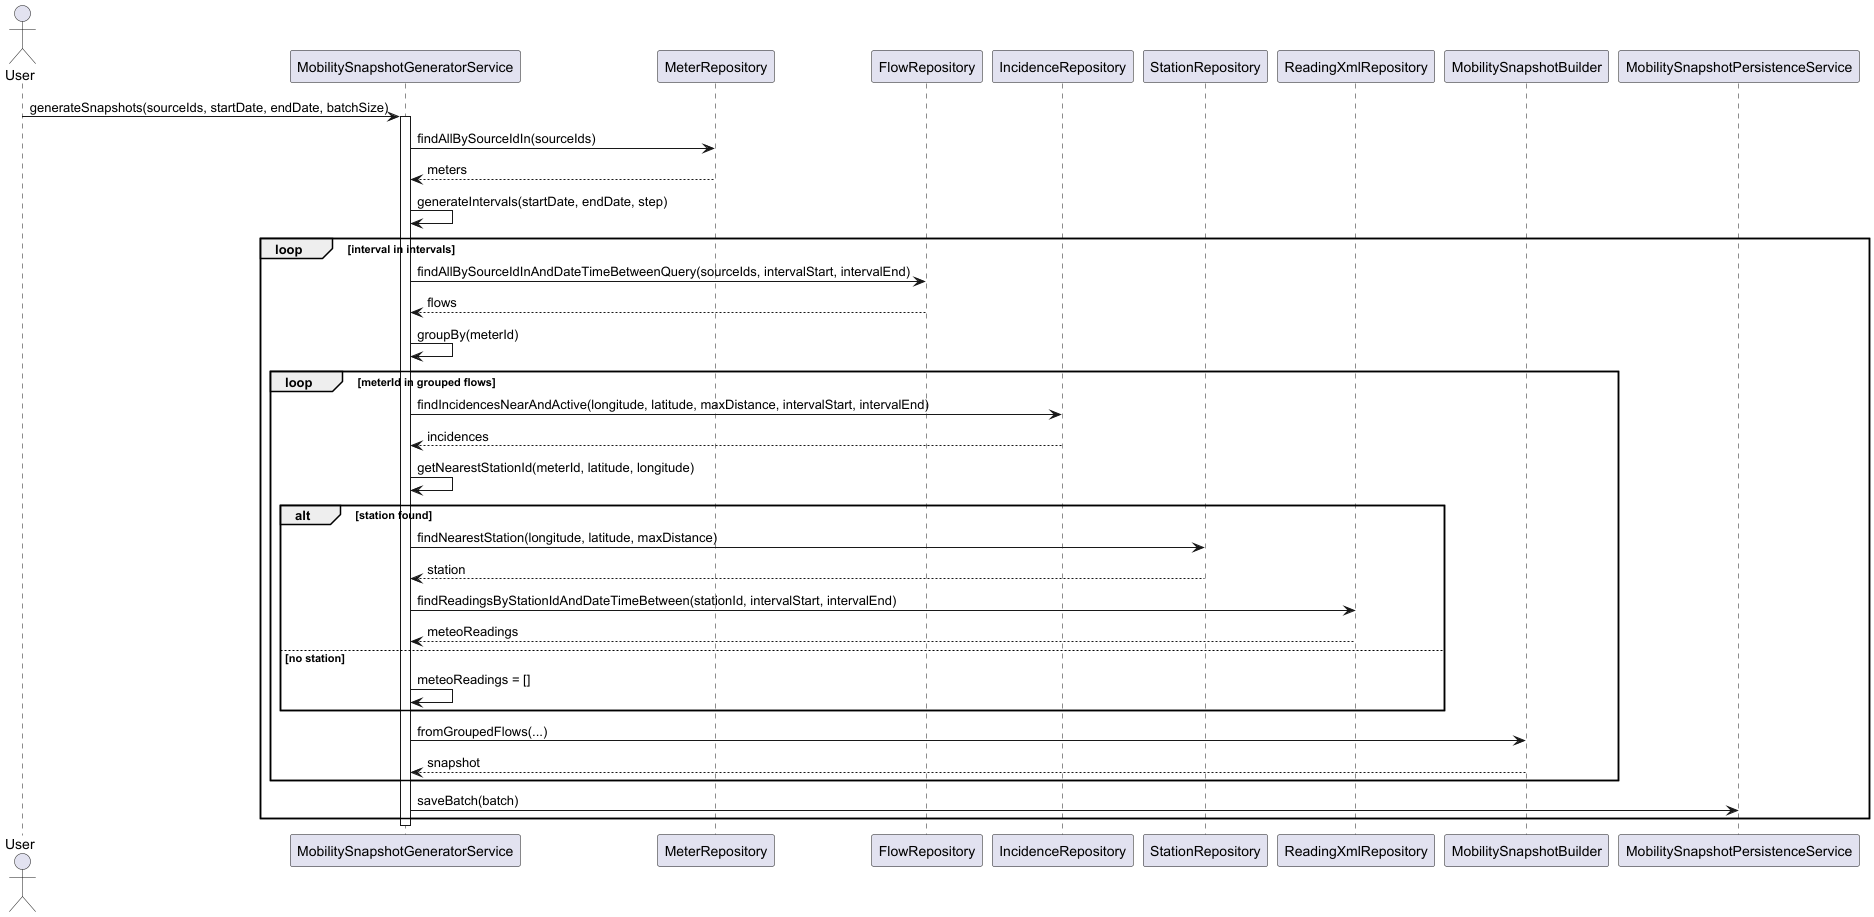
\includegraphics[width=0.95\textwidth]{includes/snapshot_generator_sequence.png}
	\caption{Diagrama de secuencia de integración y persistencia en \texttt{MobilitySnapshot}.}
	\label{fig:sequence_mobility_snapshot}
\end{figure}

El código fuente completo del componente encargado de llevar a cabo esta integración puede consultarse en el \hyperref[anexo:snapshot_generator]{Anexo~C}, donde se incluye la clase \texttt{MobilitySnapshotGeneratorService} desarrollada específicamente para este propósito.

El proceso se puede descomponer en los siguientes pasos:

\begin{enumerate}
	\item \textbf{Inicialización:} se obtienen todos los aforadores activos (\texttt{Meter}) correspondientes a los identificadores de fuente (\texttt{sourceIds}) indicados.
	\item \textbf{Ventanas temporales:} se generan intervalos de tiempo equiespaciados de 30 minutos entre las fechas de inicio y fin.
	\item \textbf{Extracción de flujos:} para cada intervalo, se recuperan todos los flujos de vehículos (\texttt{Flow}) registrados en ese rango temporal y se agrupan por aforador (\texttt{meterId}).
	\item \textbf{Procesamiento por aforador:} para cada grupo de flujos:
	\begin{itemize}
		\item Se localiza el aforador correspondiente y se calcula el número total de vehículos en la ventana.
		\item Se consultan las incidencias viales (\texttt{Incidence}) activas y geoespacialmente cercanas (500 metros) en el intervalo.
		\item Se determina la estación meteorológica más cercana usando una cache interna. Si existe, se recuperan las lecturas (\texttt{Reading}) correspondientes al intervalo temporal.
	\end{itemize}
	\item \textbf{Construcción del snapshot:} con todos los datos anteriores, se construye el objeto \texttt{MobilitySnapshot} mediante el \texttt{MobilitySnapshotBuilder}.
	\item \textbf{Persistencia por lotes:} los snapshots generados se agrupan en bloques de tamaño configurable (por defecto 500) y se guardan en la base de datos de forma transaccional.
\end{enumerate}

Para procesar los datos por ventanas temporales consecutivas, se implementa una función utilitaria llamada \texttt{generateIntervals()}, que permite dividir un periodo de tiempo en subintervalos de duración fija. Este procedimiento es fundamental en el procesamiento de datos temporales y en la agregación de observaciones como \texttt{MobilitySnapshot}.

El algoritmo se describe de la siguiente forma.

\vspace{1em}
\noindent \textbf{Descripción del funcionamiento:}
\begin{itemize}
	\item La función recibe un instante inicial (\texttt{start}), un instante final (\texttt{end}) y una duración fija (\texttt{step}).
	\item Crea una lista vacía de intervalos temporales.
	\item Mediante un bucle, se van generando pares de fechas consecutivos, avanzando de \texttt{step} en \texttt{step}.
	\item Si el último intervalo excede el tiempo final, se ajusta automáticamente para que el límite superior sea exactamente \texttt{end}.
	\item Devuelve la lista completa de intervalos como pares de fechas (\texttt{Pair<start, end>}).
\end{itemize}

\vspace{1em}
\noindent \textbf{Ejemplo práctico:}
\begin{lstlisting}[language=Kotlin, caption={Ejemplo de uso con intervalos de 30 minutos}]
	generateIntervals(
	start = 2024-01-01T00:00,
	end = 2024-01-01T01:00,
	step = Duration.ofMinutes(30)
	)
\end{lstlisting}

\noindent El resultado de este ejemplo sería:
\begin{verbatim}
	[
	(2024-01-01T00:00, 2024-01-01T00:30),
	(2024-01-01T00:30, 2024-01-01T01:00)
	]
\end{verbatim}

Este mecanismo permite particionar grandes volúmenes de datos históricos en unidades manejables, facilitando la agregación de información por tramos y reduciendo la carga computacional de los algoritmos de predicción.

Este proceso se ejecuta para todas las ventanas temporales dentro del periodo solicitado, permitiendo cubrir días, semanas o incluso meses de observaciones. Se emplean caches internas y colecciones reactivas para optimizar el rendimiento del sistema y permitir el escalado.

\subsubsection*{Consideraciones finales para la generación del dataset}

Una decisión fundamental en la construcción del dataset es la selección del intervalo temporal con el que se van a agrupar las observaciones. Este proceso, conocido como \textit{resampling temporal}, consiste en consolidar las mediciones de tráfico (\texttt{Flow}) en tramos de tiempo consecutivos y homogéneos. Esta práctica es común en el análisis de series temporales y presenta múltiples ventajas:

\begin{itemize}
	\item \textbf{Reducción de dispersión:} ayuda a evitar huecos en las series temporales, suavizando el ruido y mejorando la capacidad de generalización del modelo.
	\item \textbf{Homogeneización del dataset:} garantiza que todas las observaciones estén espaciadas en el tiempo con la misma frecuencia, lo cual es esencial para el entrenamiento supervisado.
	\item \textbf{Facilitación de integración con otras fuentes:} permite alinear los flujos con los datos meteorológicos e incidencias, los cuales pueden tener frecuencias distintas o menos regulares.
	\item \textbf{Reducción de volumen de datos:} disminuye la cantidad de registros generados, lo que mejora la eficiencia tanto en almacenamiento como en entrenamiento de modelos.
\end{itemize}

\vspace{1em}
\noindent La elección del intervalo temporal óptimo depende del equilibrio entre granularidad, capacidad computacional y riqueza informativa. Las alternativas más comunes son:

\begin{itemize}
	\item \textbf{Intervalos de 1 hora:} proporcionan una agregación suficiente para análisis diarios o semanales, son compatibles con muchos datasets públicos, pero pueden enmascarar variaciones de corto plazo (como retenciones puntuales).
	
	\item \textbf{Intervalos de 30 minutos:} capturan mejor los picos de tráfico y permiten reflejar dinámicas más rápidas (por ejemplo, alteraciones por accidentes o climatología adversa). Este intervalo ha sido el seleccionado en este proyecto como punto de partida, ya que ofrece un buen compromiso entre granularidad y manejabilidad.
	
	\item \textbf{Intervalos de 15 minutos o menos:} pueden resultar útiles si se dispone de datos de alta frecuencia, pero también pueden introducir más ruido o generar datasets demasiado voluminosos para ciertos entornos de cómputo.
\end{itemize}

\begin{table}[H]
	\centering
	\caption{Comparativa entre intervalos temporales posibles para el resampling}
	\label{tab:resample_comparison}
	\renewcommand{\arraystretch}{1.4}
	\begin{tabularx}{\textwidth}{lXXX}
		\toprule
		\textbf{Criterio} & \textbf{15 minutos} & \textbf{30 minutos} & \textbf{1 hora} \\
		\midrule
		\textbf{Granularidad} & Alta & Media & Baja \\
		\textbf{Captura de picos} & Muy buena & Buena & Limitada \\
		\textbf{Volumen de datos} & Alto & Medio & Bajo \\
		\textbf{Riesgo de ruido} & Alto & Bajo-Medio & Bajo \\
		\textbf{Compatibilidad con fuentes externas} & Menor & Alta & Alta \\
		\textbf{Recomendado para} &
		Predicción muy reactiva o microanálisis &
		Equilibrio general &
		Análisis macro o planificación \\
		\bottomrule
	\end{tabularx}
\end{table}

En la Tabla \ref{tab:resample_comparison} se puede apreciar resumidamente las consideraciones descritas anteriormente.

\vspace{1em}
\noindent \textbf{Decisión tomada:} el sistema desarrollado trabaja por defecto con ventanas de \textbf{30 minutos}. Esta elección permite capturar transiciones relevantes en la movilidad sin incrementar en exceso la complejidad del dataset. No obstante, la arquitectura del generador (\texttt{MobilitySnapshotGeneratorService}) permite modificar este parámetro fácilmente para experimentar con alternativas. Por ejemplo:

\begin{itemize}
	\item Reducir a 15 minutos si se observan patrones planos o poca sensibilidad a eventos puntuales.
	\item Aumentar a 1 hora si el volumen de datos es demasiado elevado o si se prioriza una vista agregada del tráfico.
\end{itemize}

\subsection{Arquitectura y pipeline general del proyecto}

A continuación, se presenta una descripción completa de la arquitectura y el pipeline diseñado para este proyecto, abarcando desde la recolección inicial de datos hasta la generación y validación de modelos predictivos basados en aprendizaje profundo.

Todo el proceso comienza con el artefacto \texttt{Data Collector}, un proyecto desarrollado en Kotlin utilizando el framework Spring Boot. Su función principal consiste en la construcción integral del dataset utilizado posteriormente para el entrenamiento de modelos predictivos.

En primer lugar, se ha recopilado la información meteorológica. Los datos estáticos, tales como la ubicación de las estaciones meteorológicas, se obtienen directamente mediante la API de Euskalmet proporcionada por el Gobierno Vasco. Debido a problemas técnicos en la extracción automática de las mediciones diarias, estas han sido extraídas mediante la descarga manual de un archivo ZIP del portal Open Data del Gobierno Vasco, que contiene todas las lecturas meteorológicas del año 2024.

En segundo lugar, el dataset incorpora información de aforos vehiculares proveniente de distintas fuentes, centradas exclusivamente en Bizkaia: una del Gobierno Vasco, dos de la Diputación Foral de Bizkaia y cinco del Ayuntamiento de Bilbao. La información relativa a las fuentes del Gobierno Vasco y del Ayuntamiento de Bilbao se ha extraído mediante su API de Tráfico, incluyendo tanto estaciones como mediciones e incidencias del tráfico. Por otro lado, los datos proporcionados por la Diputación Foral de Bizkaia han sido facilitados directamente mediante un acuerdo expreso con dicha institución.

Una vez obtenida y consolidada toda esta información, se almacena en una base de datos MongoDB, y posteriormente se procede a construir el dataset definitivo en la colección denominada \texttt{MobilitySnapshot}. Este proceso se describe detalladamente en secciones previas del presente capítulo.

Tras esta fase de recolección y consolidación, se entra en la etapa del proyecto principal denominado \texttt{Trafficformer Bizkaia}. Este proyecto está desarrollado en Python, utilizando librerías relevantes para el aprendizaje profundo como PyTorch. Se han implementado dos modelos predictivos principales: un modelo base \texttt{MultiLayerPerceptron} (MLP) y el modelo definitivo \texttt{Trafficformer}, basado en una arquitectura moderna de tipo Transformer.

Para gestionar los experimentos y entrenamientos, se han definido una serie de procesos específicos descritos en profundidad en el Capítulo~\ref{sec:desarrollo_comp_results}. Se han diseñado diferentes entrenamientos para evaluar ambas arquitecturas (MLP y Trafficformer) y para realizar múltiples pruebas variando hiperparámetros significativos.

Estos entrenamientos se ejecutan principalmente en notebooks Jupyter sobre una máquina local equipada con una GPU de alto rendimiento, suficiente para el entrenamiento de redes neuronales profundas. Adicionalmente, se dispone de una infraestructura preparada para realizar entrenamientos de forma escalable en la nube mediante instancias EC2 de Amazon Web Services (AWS) y utilizando imágenes AMI configuradas con soporte Nvidia.

Durante el proceso de entrenamiento y evaluación, se ha utilizado la plataforma Weight \& Biases para realizar un seguimiento detallado de los experimentos, facilitando así la elección y validación de los mejores modelos entre los 120 experimentos realizados (un experimento por cada \texttt{sourceId} y tipo de modelo).